% TODO Notation
% what is bold?
% what is caps?
% greek letters are?
% indices?
% what is a \vec? \bar? \mathbold?
% what about mathsf for each model? 
% texttt and SmallCaps for each algorithm? (\sct{Test})
% mathcal for sets
% F_{u,v | Y=0} --> P[u,v | Y=0]
% i wouldn't use commas for A_{i,j} just A_{ij}
% no 'iid' or 'd' above \sim
% assignment vector is \tau, 

% TODO maybe we don't need Table 1? if we need space we can put it in appendix, for example?
% Jesus thinks its useful
% JA: I do not necessarily mean having a table, but the paper does need some place to state basics about notation (especially subindexes, see comment below)

% TODO: It'll be nice to define notation somewhere before this section. In particular, be clear about subindexes, especially for rows of X since it is not very intuitive what is X_i. 

% \begin{table}
% \caption{Notations and symbols used in this paper}\label{tab1}
% \begin{center}
% \begin{tabular}{|@{}l|c@{}|}
% \hline
% Symbols & Description\\
% \hline
% $[n]$ & $\{1, 2, \ldots, n\}$\\
% $\mathcal{G}$ & Graph\\
% $n$ & Number of nodes\\
% $\A$ & Adjacency matrix\\
% $\A_i$ & $i$-th row of $\A$\\
% $\A_{ij}$ & $(i,j)$ entry of $\A$\\
% $\A^{(l)}$ & $l$-th element in sequence of $\A$\\
% $\Pbf$ & Edge connectivity probability matrix\\
% $\B$ & Block connectivity probability matrix\\
% $\vec{\tau}$ & Vertex community assignment vector\\
% $\M$ & Edge community assignment matrix\\
% $\X$ & Latent position matrix\\
% $\hat{\X}$ & Estimated latent position matrix\\
% \hline
% \end{tabular}
% \end{center}
% \end{table}

\begin{table}
\caption{Notations and symbols used in this paper}\label{tab1}
\begin{center}
\begin{tabular}{|@{}l|c@{}|@{}l|c@{}|}
\hline
Symbols & Description & Symbols & Description\\
\hline
$[n]$ & $\{1, 2, \ldots, n\}$ & $\Pbf$ & Edge connectivity probability matrix\\
$\mathcal{G}$ & Graph & $\B$ & Block connectivity probability matrix\\
$n$ & Number of nodes & $\vec{\tau}$ & Vertex community assignment vector\\
$\A$ & Adjacency matrix & $\M$ & Edge community assignment matrix\\
$\A_i$ & $i$-th row of $\A$ & $\X$ & Latent position matrix\\
$\A_{ij}$ & $(i,j)$ entry of $\A$ & $\hat{\X}$ & Estimated latent position matrix\\
$\A^{(l)}$ & $l$-th element in sequence of $\A$ & &\\
\hline
\end{tabular}
\end{center}
\end{table}

\section{Statistical Models}\label{sec:models}
Connectomes can be modelled using statistical models designed for network data \cite{ goldenberg2010survey, kolaczyk2014statistical}. Statistical models consider the entire network as a random variable, including the inherent structure, dependencies within networks, and the noise in observed data. 
Thus, statistical models can formalize detecting similarities or differences for each of the representations in Section \ref{sec:representations}.
This section provides an overview of many statistical models for network data, including those designed for representing single and multiple networks. 

Section \ref{sec:single_graph_models} provides an overview of single graph models that have been extensively studied as well as recently introduced models in the order of least to greatest complexity. Figure \ref{fig:models}a shows the relationship between all the single graph models presented in this paper. Section \ref{sec:multi_graph_models} provides an overview of some models for multiple networks. While other statistical models for multiple network data exist \cite{zhang2018network, wang2019joint, nielsen2018multiple, Durante2017-fz}, we focus on  some recent models that are used in spectral inference for connectomics data. In Appendix \ref{sec:model_extensions}, we describe some extensions to these models. 

\begin{figure}
    \centering
    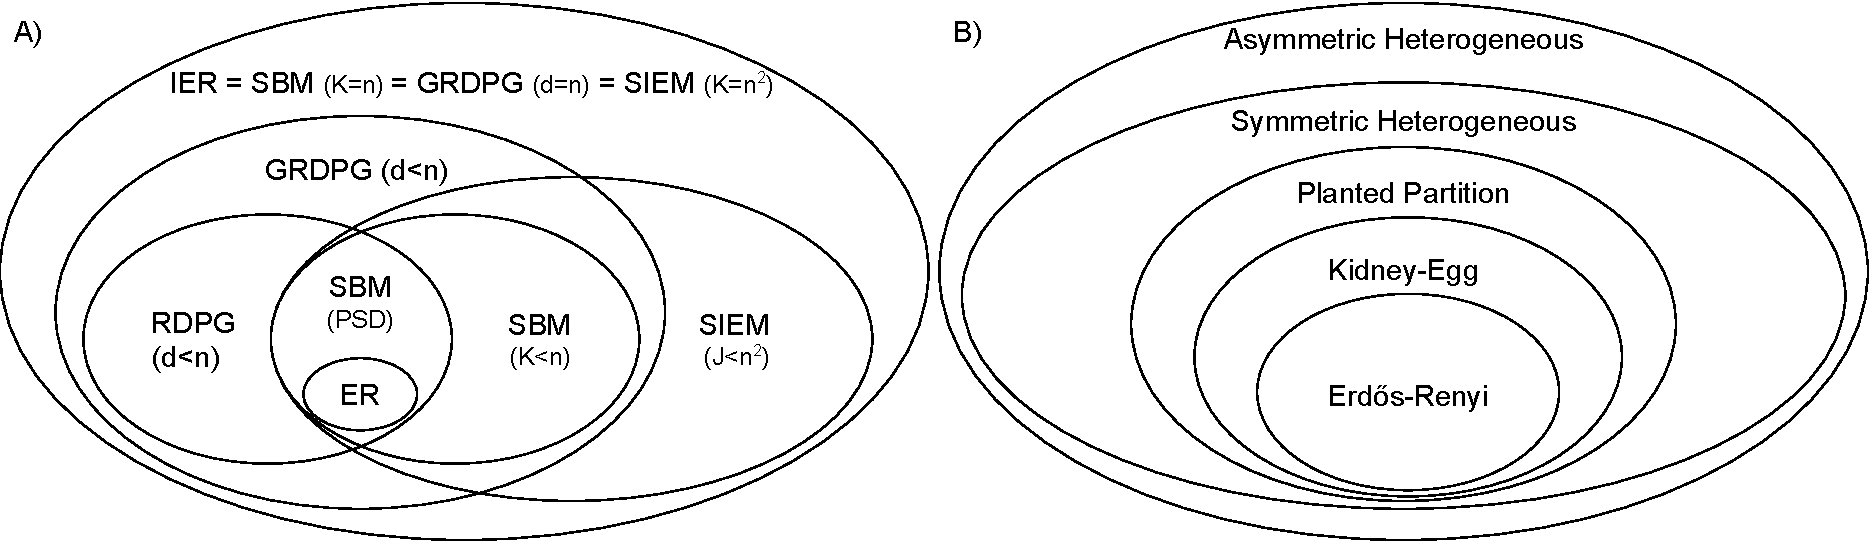
\includegraphics[width=\textwidth]{figures/dnd/models_combined}
    \caption{\textbf{Hierarchical Relationships of Statistical Models} 
    \textbf{(a)} Relationships among all the single-graph statistical models. Erd\H os-R\'enyi ($\er$) model is a stochastic block model ($\sbm$) with one community. $\sbm$ with a positive semidefinite block probability matrix $\B$ is also a random dot product graph ($\rdpg$). Any $\sbm$, $\rdpg$, and some structured independent edge model ($\siem$) can be represented as $d$-dimensional generalized random dot product graph ($\grdpg$) with $d$ less than number of vertices $n$. Inhomogenous Erd\H os-R\'enyi ($\ier$) model is equivalent to a $n$-block $\sbm$, $n$-dimensional $\grdpg$, and $n^2$-group $\siem$.
    \textbf{(b)} Relationships among the two-block $\sbm$ models. The most complex model is the asymmetric heterogeneous $\sbm$, and the simplest model is the $\er$, which is a degenerate case of 2-block $\sbm$.}
    \label{fig:models}
\end{figure}

\subsection{Single Graph Models}\label{sec:single_graph_models}
% TODONE: This section seems very short. Maybe you can add something to motivate why do we care about the ER model. For example, saying that this model is completely specified by its expected density, and it is useful to understand the effect of the number of edges in certain network phenomena (maybe cite \cite{Rukhin2010}). 
\subsubsection{Erd\H os-R\'enyi Random Graphs (ER)}\label{sec:uer}
The simplest random graph model is the $\mathsf{Erd\ddot{o}s-R\acute{e}nyi~(ER)}$ model \cite{Erdos1959-zf}. For a given set of $n$ vertices, each distinct pair of vertices are connected independently with probability $p \in [0, 1]$. Specifically, $\A \sim\er_n(p)$ if $\A$ has entries $\A_{ij}\sim\bern(p)$ for $i, j \in [n]$. While the $\er$ model is not representative of real data, it has been studied extensively since many of its properties can be solved exactly  \cite{newman2003random,Rukhin2010}.  
%Figure \ref{fig:er_sbm_example} shows an example of an $\er$ graph.

\subsubsection{Stochastic Block Model (SBM)}\label{sec:usbm}
First introduced in \cite{holland1983stochastic}, $\sbm$ is a model that can produce graphs with vertices grouped into $K$ communities \cite{Rohe2011-ha,sussman2012consistent,Wasserman1987-tw}. There are two simple variations of the $\sbm$ in which the vertex assignment vector $\vec \tau \in \left\{1, \hdots, K\right\}^n$ is known \textit{a priori}, and where $\vec \tau$ is not known. 
In both cases, a symmetric $K \times K$ block connectivity probability matrix $\B$ with entries in $[0,1]^{K \times K}$ governs the probability of an edge between vertices given their block memberships. 

% TODONE : check consistency in the notation of Bernoulli
% TODO when tau is known, it is still a parameter, right? if so, i don't think the below sentences are exactly right in terms of the word 'parameterized'. i kinda think of \pi existing either way, and in the a priori, we condition on sampling tau, and the a posteriori, we do not.  might be clearer that way? possibly discuss with jesus?
% ja: I agree that tau is a parameter in the a priori model. in the a posteriori model, the parameter is \pi.
If $\vec \tau \in \left\{1, \hdots, K\right\}^n$ is known \textit{a priori}, the \textit{a priori} $\sbm$ is parametrized only by the block connectivity matrix $\B$, and the model is $\A \sim \sbm_n(\vec \tau,\B)$ if $\A$ has entries $\A_{ij} \sim \bern(\B_{kl})$ where $\tau_i = k, \tau_j = l$, for $i, j \in [n]$, and $k, l \in [K]$. In the case where $\vec \tau$ is not known, the \textit{a posteriori} $\sbm$ is additionally parameterized by a block membership probability vector $\vec{\pi} = [\pi_1,\dots,\pi_K]^\top$ on the probability simplex.
The model is $\A \sim \sbm_n(\vec \pi,\B)$ if $\A$ has entries $\A_{ij} \big | k=\tau_i, l=\tau_j \sim \bern(\B_{kl})$, where $\tau_i {\sim} \multinomial(\vec \pi)$ for $i = 1, \hdots, n$. 

% TODONE: Does homophily require a > b? I think the definition of homophily is that people connect with similar people more often. https://en.wikipedia.org/wiki/Homophily
% TODONE i agree with the above, in homophily, a>b.  might need to change the name.  maybe what we call symmetric homophilly is really planted partition? check with jesus.
% ja: yes, it is planted partition https://www.cs.columbia.edu/~djhsu/AML/lectures/planted.md.handout.pdf
% but then asymmetric homophily is nothing in particular

Throughout the context of this paper, we will focus particularly on a few variations of the two-block $\sbm$ ($K=2$) with block connectivity matrix $\B = \begin{bmatrix}a & b \\ c & d \end{bmatrix}$, abbreviated as $\B = [a, b; c, d]$. The common variants include:
\begin{enumerate}
    \item $\mathsf{Kidney-Egg}$: $b = c = d$. In this model, one of the blocks has edges with a different probability than the others, but the remaining blocks are homogeneous, where $a \neq b$. Furthermore, when $b > a$, the model is referred to as core-periphery $\sbm$.
    \item $\mathsf{Planted~Partition}$: $a = d$ and $b = c$. In this model, the within-block edges share a common probability $a$, and the between-block edges share a common probability $b$, where $a \neq b$.
    % TODONE: Earlier you said that you were only going to consider undirected edges. Then it is not possible to have asymmetric B. You probably need to consider directed networks and explain that this model is for directed, or remove this
    % TODONE agreed, explain relevant for undirected.
    %\item $\mathsf{Asymmetric~ Homophily}$: $\B = \begin{bmatrix}a & b \\ c & a \end{bmatrix}$. In this block model, the within-block edges share a common probability $a$, but the between-block edges have different probabilities, where $a \neq b \neq c$.
    % TODONE: Same as before, if you only consider undirected then there is no need to have symmetric and assymetric
    % Assymetric heterogenous is used in apps so keeping this.
    \item $\mathsf{Symmetric~ Heterogeneous}$: $b = c$. In this model, the between-block edges share a common probability $b$, but the within-block edges have a disparate probabilities, where $a \neq b \neq d$. 
    \item $\mathsf{Asymmetric~ Heterogeneous}$: $a \neq b \neq c \neq d$. In this directed model, every block has a unique probability.
    % TODONE can we use 'd' for lower right?  basically, in all cases, B=[a, b; c, d].  in the different models, different parameters are equal/not equal to each other. this might be an easier and more concise way to explain all the different models.
    % TODONE: I think assortativity and homophily are the same thing? http://tuvalu.santafe.edu/~aaronc/courses/5352/fall2013/csci5352_2013_L5.pdf
    % TODO@jv: this directed one is kept since we use this model in apps
    \item $\mathsf{Erd\ddot{o}s-R\acute{e}nyi}$: $a=b=c=d$. In this degenerate model, all blocks have a common probability, and the partitioning is irrelevant. 
    \item $\mathsf{Homophilic/Assortative/Affinity}$: $a, d > b, c$. In this model, the within-block probabilities are greater than cross-block probabilities.
    \item $\mathsf{Disassortative}$: $ b, c > a, d$. In this model, the cross-block probabilities are greater than the within-block probabilities.
\end{enumerate}
Figure \ref{fig:models}b summarizes the relationships of $\sbm$ models.

% TODONE i'd like ER as a special case in the enumerated ones, where a=b=c=d.
% TODO maybe add ER to fig 4? and affinity/assortative.  and we should state what planted partition model is (it is what you mean when you wrote symmetic homophylic.  also might want to state what dissortative is. and add to figure. 
% TODO@jv : not sure how i can draw the appropriate circles for homophilic and disassortative. too many overlaps?

%, and Figure \ref{fig:er_sbm_example} shows an example of a planted partition $\sbm$ graph. 
% \begin{figure}
%     \centering
%     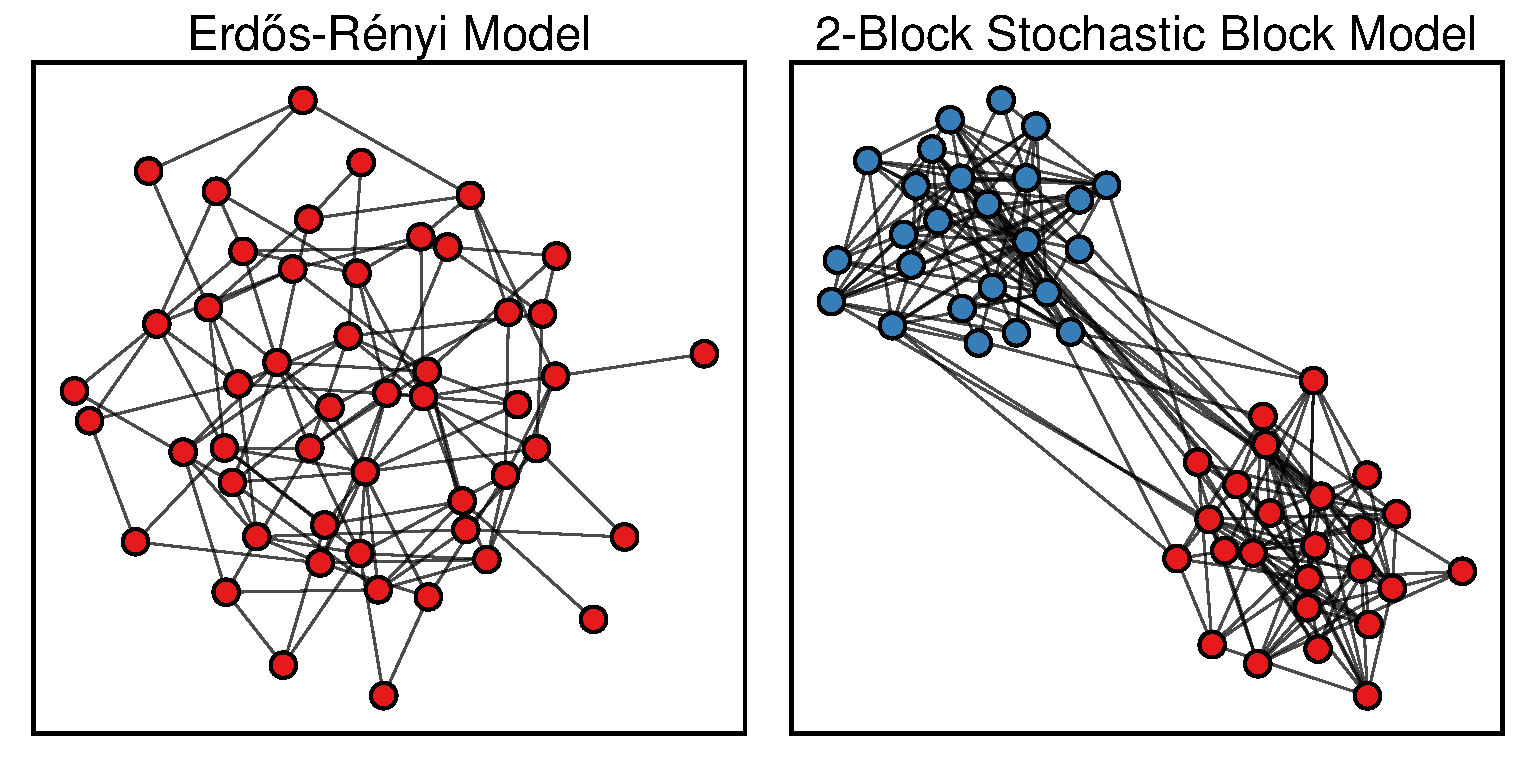
\includegraphics[width=.65\textwidth]{figures/dnd/er_sbm_example}
%     \caption{
%     \textbf{Simulated Graphs From an $\er$ and $\sbm$ Models.}
%     \textit{(Left)} A random graph from ER model with $n = 50$ and $p = 0.1$. \textit{(Right)} A random graph from a $\mathsf{Symmetric~ Homophilic} \sbm$ model with $n = 50$, $\vec{\pi} = [0.5, 0.5]$, and $B = [0.25, 0.025;0.025, 0.25]$. Blue and red dots represent block memberships.
%     }
%     \label{fig:er_sbm_example}
% \end{figure}

\subsubsection{Structured Independent Edge Model (SIEM)}\label{sec:usiem}
% TODONE: I suggest to change communities to clusters here. Communities are usually defined in terms of a node property. Here it is not possible to have the same property for an edge because there is only one edge observation.
$\siem$ is a generalization of $\sbm$ that produces graphs in which edges are grouped into one of $K$ clusters. Analogous to the vertex assignment vector of the \textit{a priori} $\sbm$, the $\siem$ features an edge community assignment matrix $\M \in \left\{1, \hdots, K\right\}^{n \times n}$ which is known \textit{a priori}. Given the community assignment matrix $\M$, the $\siem$ is $\A \sim \siem_n(\M, \vec p)$ if $\A_{ij} {\sim}\bern(p_k)$ where $\M_{ij} = k$, for $i, j \in [n]$ and $k \in [K]$. $\vec p = [p_1, \hdots, p_K]^\top \in [0, 1]^K$ is the edge probability vector which governs the probability of an edge between vertices. 

% TODONE: In my opinion, the a posteriori SIEM is not very interesting for a single graph since it will essentially look like an ER model if the membership assignments are random. Also, the term block probablity seems weird since there are no blocks on this model. I think it could be interesting for multiple networks in which the clusters can be identified, but unless there is a motivating example in the paper, my suggestion would be to remove the a posteriori SIEM

% In the case where $\M$ is not known, the \textit{a posteriori} $\siem$ is additionally parameterized by a block membership probability vector $\vec \pi = [\pi_1, \hdots, \pi_K]^\top$ on the probability simplex.
% The model is $\A \sim \siem_n(\vec \pi, \vec p)$ if $\A_{ij} \big| \M_{ij} = k \sim \bern(p_k)$ where $\M_{ij} {\sim} \multinomial (\vec \pi)$, for all $i, j \in [n]$. 

The \textit{a priori} $\sbm$ is a special case of $\siem$ in which edges are assigned to blocks $\M$ which respect the vertex assignment vector $\vec \tau$. For the purposes of this paper, we will consider a case that frequently comes up in neuroimaging, the $\mathsf{Homotopic~ SIEM}$, in which each vertex has a matched ``pair'' amongst other vertices. The edges corresponding to a pair $\M_{ij} = 2$ where $(v_i, v_j)$ are a pair of vertices sharing a property, and the edges corresponding to a non-pair are $\M_{ij} = 1$. A matched pair of vertices, for instance, could be homotopic brain regions (two brain regions with similar function but in opposing hemispheres of the brain).
% TODONE@jv i don't think that is what we mean.  we mean that M_{ij} is big when (i,j) are paired, relative to when (i,j) are not paired. but above you wrote equal.
% the M matrix is just arbitrary labels; they don't mean anything, so I don't know what you mean. I updated to reflect 2 and 1, for example, to be more specific but they could really be anything (ie, 1 and 2 would be the same as long as you respectively flip p2 and p1).
% TODONE@eb: let's remove the term 'a priori SIEM', there is only 1 kind of SIEM.  let's remove homotopic SIEM, it is homotopic SBM.  talk about homophylic

\subsubsection{Random Dot Product Graphs (RDPG)}\label{sec:rdpg}
$\rdpg$ belongs to the class of latent position random graphs \cite{hoff2002latent}. In a latent position graph, every vertex has associated to it a (typically unobserved) \textit{latent position} in some space $\mathcal{X}$, and the probability of connection between vertices $i$ and $j$ are given by a link function. In $\rdpg$, the space $\mathcal{X}$ is a constrained subspace of Euclidean space $\RR^d$ and the link function is the dot product \cite{Young2007-vu,scheinerman2010modeling,Sussman2014-zq}. Thus, in a $d-$dimensional $\rdpg$ with $n$ vertices, the matrix $\X\in \RR^{n\times d}$ whose rows are the latent positions, and the matrix of connection probabilities is given by $\Pbf=\X\X^\top$, which is positive semidefinite. The model is $\A\sim \rdpg_n(\X)$ if the adjacency matrix $\A$ has entries $\A_{ij} \sim \bern(\X_i\X_j^\top)$.
Subsequent inference tasks include community detection \cite{sussman2012consistent}, vertex classification \cite{tang2013}, or two-sample hypothesis testing for graphs with matched and non-matched vertices for a pair of graphs  \cite{priebe2019two,tang2017nonparametric,tang2017semiparametric}.
% TODONE: Related to earlier comment about notation. When you have X_i, is it a matrix or a vector? If it is a matrix, then it is fine, but you need to indicate it in the notation. If it is a vector, then you need to do X_i^T X_j to get a real number, otherwise you get a d x d matrix. I think some readers can figure it out from the context, but I find difficult to read papers that don't define that explicitly.

The $\rdpg$ is a flexible model, and other models of interest can be seen as special cases of the $\rdpg$. A $\sbm$ whose block connectivity matrix $\B$ is positive semi-definite is a $\rdpg$ with $K$ distinct latent positions. Thus, a $\sbm$ with $K$ blocks can be represented with a latent position matrix $\X\in\RR^{n\times d}$, with $d\leq K$, where there are only $K$ different rows of $\X$, and letting $\X_{\mathcal{U}}\in\RR^{K\times d}$ be the matrix with the subset of the rows $\mathcal{U}$ where each row is the latent position for a block, then the block connectivity matrix is $\B= \X_\mathcal{U}\X_\mathcal{U}^\top \in\RR^{K\times K}$. More generally, the $\rdpg$ can represent other models with more complex structures, such as mixed memberships \cite{Airoldi2008-tp} or hierarchical communities \cite{Lyzinski2017-cq}.

% TODONE: I updated this paragraph a bit (no need to do anything) to make the notation more consistent with the RDPG definition and make the definition more precise. Also, I think mentioning again the ER is not very informative since it was already mentioned that the ER is an SBM. Instead I named some generalizations of the SBM

\subsubsection{Generalized Random Dot Product Graphs (GRDPG)}\label{sec:grdpg}
Unlike $\rdpg$ model, $\grdpg$ does not assume that $\Pbf$ is a positive semidefinite probability matrix  \cite{rubin2017statistical}. In this model, the edge probability matrix is given by $\Pbf=\X \I_{pq}\X^\top$, and $\A\sim\grdpg_n(
\X, p, q)$ if $\A_{ij}\sim\bern(\X_i\I_{pq}\X_j^\top)$ where $\I_{pq}=\textrm{diag}(1, \ldots, 1, -1, \ldots, -1)$  with $p$ ones followed by $q$ minus ones on its diagonal, and where $p \geq 1$ and $q \geq 0$ are two integers satisfying $p + q = d$.
% TODO i find this notation confusing.  can we just write P = X Y^T?  jesus will know.
% ja: In my opinion, writing it with X and Y will be a bit more confusing because that doesn't guarantee that P is symmetric, so you need to put some constraints on Y. I guess it is a bit confusing but it is the simplest notation I can think of. Maybe adding a note that with this model, we can have any low rank matrix and write P = Q\Lambda Q^T for some eigenvectors Q size nxd and eigenvalues \Lambda d x d?
% jv: what about X X\T - Y Y\T, which is what the notation is doing, just in an obscure way?
% ja: that is fine I think, but that needs to specify that X is a  n x d_1 matrix and  Y is  n x d_2 with d_1 + d_2 = d, and [X, Y] is a full rank matrix. Otherwise, this formulation can be over-parameterizing the model

The $\grdpg$ generalizes all of the previous models. When $q=0$, $\grdpg$ reduces to a $\rdpg$ model. To represent any $\sbm$ as $\grdpg$, let $p\geq 1, q\geq 0$ be the number of positive and negative eigenvalues of the block connectivity matrix $\B\in\RR^{K\times K}$, respectively. The block matrix can be represented as $\B = \X_\mathcal{U}\I_{pq}\X_\mathcal{U}^\top$.

% TODONE: Check consistency on the symbol for transpose. Some places have $X^T$ and others have $X^\top$

\subsubsection{Inhomogenous Erd\H os-R\'enyi Random Graphs (IER)}\label{sec:uierrg}
The $\mathsf{Inhomogenous~Erd\ddot{o}s-R\acute{e}nyi~(IER)}$ is a model where each pair of nodes has a unique probability of an edge existing between the two, and is therefore the most general independent edge model. For a given set of $n$ vertices, the $\ier$ is parametrized by a matrix $\Pbf \in [0, 1]^{n \times n}$, where $\Pbf_{ij}$ is the probability of an edge connecting vertices $v_i, v_j$ where $i, j \in [n]$. That is, $\A \sim \ier_n(\Pbf)$ if $\A$ has entries $\A_{ij}\sim \bern(\Pbf_{ij})$ for $i, j \in [n]$. $\ier$ cannot be estimated from a single graph, as there are $n\choose 2$ unknowns (the probabilities) with $n\choose 2$ total observations (the edges).

% TODONE the above is true only for directed loopy graphs.  please specify. 

Note that all single graph models are special cases of $\ier$. Additionally, $\sbm$ with $K=n$, $\siem$ with $K=n^2$, and $\grdpg$ with $d=n$ are equivalent to an $\ier$ model.

\subsection{Multiple Graph Models}\label{sec:multi_graph_models}

% TODONE the below confuses models with estimation of latent positions.  the model has nothing to do with embedding or learning, please clarify.
A common idea in statistical models for multiple graphs is a shared latent space that contain structural information common to all graphs. The two models presented in this section constrain the shared latent space in different ways to describe the heterogeneity in graphs, which results in sensitivity to different kinds of heterogeneity. The advantages and disadvantages of each model are highlighted in Section \ref{sec:multi_app}.

In the following models, consider a sample of $m$ observed graphs $\mathcal{G}^{(1)}, \mathcal{G}^{(2)}, \ldots, \mathcal{G}^{(m)}$  and their associated adjacency matrices, $\A^{(1)}, \A^{(2)}, \ldots, \A^{(m)}\in\RR^{n\times n}$ with $n$ vertices that are identical and shared across all graphs. 

\subsubsection{Joint Random Dot Product Graphs (JRDPG)}
In this model, we consider a collection of $m$ $\rdpg$s all with the same generating latent positions. Similar to a $\rdpg$, given an appropriately constrained Euclidean subspace $\RR^d$, the model is parameterized by a latent positions matrix $\X\in\RR^{n\times d}$ where $d \ll n$. The model is $\left(\A^{(1)}, \A^{(2)}, \ldots, \A^{(m)}\right)\sim \jrdpg(\X)$ where $\A_{ij}^{(l)}\sim \bern(\X_i\X_j^\top)$ for all $i, j \in [n]$ and $l\in [m]$. Each graph has marginal distribution $\A^{(l)}\sim\rdpg(\X)$ for all $l \in [m]$, meaning that the matrices $\A^{(1)}, \ldots,\A^{(m)}$ are conditionally independent given $\X$ \cite{athreya2017statistical,levin2017central}. While the model assumes that the latent positions for the graphs are the same, we note that this assumption is likely violated in heterogeneous networks, but still remains a very useful model as shown in Section \ref{sec:multi_app}.

\subsubsection{Common Subspace Independent-Edge Model (COSIE)} \label{sec:cosie}
In this model, the heterogeneous networks are described via a shared latent structure on the vertices, but also permits sufficient heterogeneity via individual matrices for each graph  \cite{arroyo2019inference}.
The model is parameterized by a  matrix $\V\in\RR^{n\times d}$ with orthonormal columns, 
where $n$ is the number of vertices and $d\ll n$, and  symmetric individual score matrices $\R^{(i)}\in\RR^{d\times d}$. The matrix $\V$ characterizes a low-rank common subspace, and is related to the latent positions for the vertices, and the score matrices incorporate individual differences to model the heterogeneity of the graphs. The model is denoted by $\left(\A^{(1)}, \ldots, \A^{(m)}\right)\sim \cosie(\V; \R^{(1)}, \ldots, \R^{(m)})$ where $\A_{ij}^{(l)} \sim \bern(\mathbf{P}^{(l)}_{ij})$ for all $i, j\in [n], i < j$, and $\mathbf{P}^{(l)}=\V\R^{(l)}\V^\top$. This factorization of the expected adjacency matrices is related to other decompositions for multiple matrices into population singular vectors or eigenvectors and individual parameters \cite{afshin2012enhancing,crainiceanu2011population,lock2013joint,wang2019common}.
% TODONE jesus, can we mention here the relationship between COSIE model, and GCCA, the SVD like thing, and maybe JIVE?

\subsubsection{Correlated Models} \label{sec:correlated-graphs}

% TODO: This part probably needs some introduction to transition and connect with the rest of the paper. Note that in the introduction of this section only the embeddings are discussed

Finally, we are interested in graph models for a pair of graphs, $\mathcal{G}_1$ and $\mathcal{G}_2$, where the two graphs are said to be correlated; that is, the edges adjoining incident vertices have a non-zero correlation. Correlated graph models have numerous applications, such as when a graph is estimated repeatedly for the same source at different points in time.

% TODONE: I think that these two sections have essentially the same information, and the P,Q model is only more general. Therefore I suggest to maybe merge them into one and explain that correlted RDPG is when $P = Q = XX^T$?
% TODONE agreed.
% TODONE: I updated this section because the definition was very confusing and the notation was not consistent with other parts
\paragraph{Correlated $(\Pbf,\Q)$}

The $\mathbf{R}$-correlated $(\Pbf, \Q)$ model \cite{lyzinski2017matchability} with parameters $\mathbf{R}, \Pbf, \Q\in[0,1]^{n\times n}$, denoted as $\mathrm{CorrER}(\Pbf, \Q, \mathbf{R})$, produces two graphs $\mathcal{G}_1$ and $\mathcal{G}_2$ with adjacency matrices $\A^{(1)}, \A^{(2)}$ such that each graph is marginally an inhomogeneous Erd\H{o}s-R\'enyi with $\A^{(1)} \sim \ier(\Pbf)$, $\A^{(2)}\sim \ier(\Q)$, but the  pairs of corresponding edges have Pearson correlation  encoded in the matrix $\mathbf{R}$ such that 
$$\mathbf{R}_{ij} = \text{Corr}(\A^{(1)}, \A^{(2)})= \frac{\mathbb{P}(\A^{(1)}_{ij}=\A^{(2)}_{ij}=1)-\Pbf_{ij}\Q_{ij}}{\sqrt{\Pbf_{ij}(1-\Pbf_{ij}) \Q_{ij}(1-\Q_{ij})}}.$$
When $\Pbf$ and $\Q$ are different, there are restrictions in the values that the correlation matrix $\mathbf{R}$ can take. In particular, if $\Pbf_{ij}\neq\Q_{ij}$  and $\Pbf>\Q$, then $\mathbf{R}_{ij}\leq \sqrt{\frac{\Q_{ij}(1-\Q_{ij})}{\Pbf_{ij}(1-\Pbf_{ij})}}$ \cite{lyzinski2017matchability}.


%, where $\mathbb E [\A^{(1)}] = \Pbf$, and $\mathbb E[\A^{(2)}] = \Q$, and each edge of $\mathcal{G}_1$ has a single corresponding edge in $\mathcal{G}_2$ to which it is correlated (but has a different probability). Specifically, let $\left(\A_{ij}^{(1)}, \A_{ij}^{(2)}\right) \sim F\left(\Pbf_{ij}, \Q_{ij}, r'_{ij}(\rho_{ij})\right)$, where $\rho_{ij}$ is chosen such that $\left(\A_{ij}^{(1)}, \A_{ij}^{(2)}\right)$ has a valid distribution for all $i, j \in [n]$. That is, $\rho_{ij}$ is chosen such that $r'_{ij}(\rho_{ij}) = (1 - p_{ij})(1 - q_{ij}) + \rho_{ij}\sqrt{p_{ij}^{(1)}q_{ij}(1 - p_{ij})(1 - q_{ij})}$, and:
% \begin{align*}
%     \zeta_{ij, ab} = \mathbb P\left(\left(A_{ij}^{(1)}, A_{ij}^{(2)}\right) = (a, b)\right) &= \begin{cases}
%         r'_{ij}(\rho_{ij}) & a, b = 0 \\
%         1 - q_{ij} - r'_{ij}(\rho_{ij}) & a = 1, b = 0 \\
%         1 - p_{ij} - r'_{ij}(\rho_{ij})& a = 0, b = 1 \\
%         r'_{ij}(\rho_{ij}) + p_{ij} + q_{ij} - 1& a, b = 1
%     \end{cases}
% \end{align*}
% is such that all the sum of the probabilities each sum to $1$, and all probabilities are at most $1$ and at least $0$. We write that $\A_1, \A_2 \sim \pmb \rho(\Pbf, \Q)$ if $\left(A_{ij}^{(1)}, A_{ij}^{(2)}\right) \sim F\left(p_{ij}, q_{ij}, r'(\rho_{ij})\right)$ as above for all $i, j \in [n]$, where $\pmb \rho$ is a valid matrix of correlations as defined above.

We are interested particularly in two special cases of the $\mathrm{CorrER}(\Pbf, \pmb Q, \pmb R)$:
\begin{enumerate}
    \item The $\rho$-correlated $\rdpg$ model arises when $\Pbf = \Q=\X\X^\top$ for some latent position matrix $\X \in \RR^{n \times d}$  as in Section \ref{sec:rdpg}, and $\pmb R = \rho \pmb 1_{n \times n}$ (that is, the matrix of edge correlations $\pmb R$ has only a single unique entry $\rho\geq 0$). We say that $\A_1, \A_2 \sim \rho\rdpg(\X)$.
    \item The $\rho$-correlated $\er$ model arises in the case where $\Pbf = \Q = p\pmb 1_{n \times n}$ (i.e.,  the probability matrix has a single unique entry $p>0$), and $\pmb R = \rho\pmb 1_{n \times n}$ (as above, the matrix of correlations has a single unique entry). We say that $\A_1, \A_2 \sim \rho\er(p)$.
\end{enumerate}